\section{Angewandte Ansätze für die Erkennung von Design Patterns}

Bei der Erkennung von Design Patterns in Quellcode wurden verschiedene Verfahren entwickelt, die auf unterschiedlichen Methoden beruhen, um das gesetzte Ziel zu erreichen.
Yarahmadi et al.~führten in ihrer Arbeit eine Untersuchung über die Methoden, die angewandt worden sind, um Design Patterns in Quellcode zu erkennen, durch und kategorisierten diese~\cite[S. 5805]{yarahmadi2020design}.

\begin{figure}[h]
    \centering
    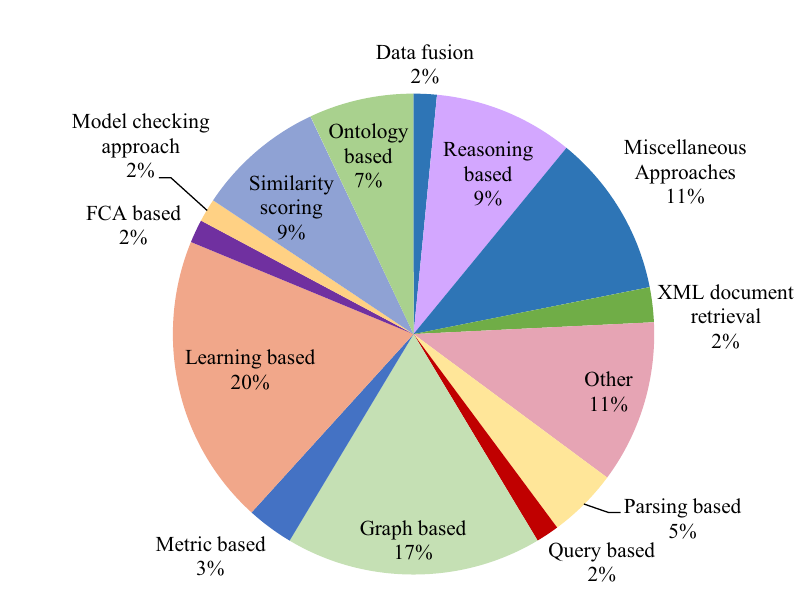
\includegraphics[scale=0.5]{figures/approches_distribution.png}
    \caption{Verteilung der Kategorien der Ansätze für die Erkennung von Design Patterns in Quellcode}
    \label{fig:approach_dist}
\end{figure}

Wie aus Figur~\ref{fig:approach_dist} zu entnehmen ist, wurden die entwickelten Prozesse von Yarahmadi et al. auf eine begrenzte Menge an Kategorien eingestuft.
In dieser Sektion der Arbeit werden die vier größten Kategorien aus Figur~\ref{fig:approach_dist} genauer erläutert und es werden exemplarische Arbeiten diskutiert, die zu der jeweilige Kategorie zugeordnet werden.

\subsection{Graphen-basierende Ansätze}

Die Methodik der Reduktion stellt in der Berechenbarkeitstheorie einen Ansatz dar, um Lösungswege für neue unbekannte Probleme zu entwickeln. Dabei wird durch einen Algorithmus das unbekannte Problem in ein bereits gelöstes Problem, dessen Lösungsweg schon vorhanden ist, umgewandelt.
In Graphen-basierenden Methoden für die Erkennung von Design Pattern in Quellcode wird diese angewendet, um Quellcode in Graphen zu transformieren und diese Graphen werden als Eingabe für diverse Graphenalgorithmen verwendet.

\pagebreak

Formell betrachtet ist ein Graph definiert als~\cite[S. 9]{Siu1998IntroductionTG}:
\begin{align*}
& \text{G} = \{V(G), E(G)\}
&\\
&\text{mit}
&\\
&G : \text{der zu betrachtende Graph}\\
&V (G): \text{Nicht leere Menge von Knoten in G}\\
&E (G): \text{Menge an ungeordneten Tupeln von distinkten Elementen von V (G)}
\end{align*}

Der Quellcode selbst ist als roher Text zu betrachten, welcher verschiedene Entitäten wie Klassen, Objekte und Schnittstellen beinhaltet und definiert, wie diese miteinander interagieren. Als Graph $G$ werden die Entitäten aus dem Quellcode als Knoten $V (G)$ und 
die Relationen und Interaktionen wie Vererbung oder Methodenaufrufe werden als Kanten $E (G)$ dargestellt.
Hierbei stellt Unified Modeling Language (UML) eine in der Software-Entwicklung verbreitete Modellierungssprache dar und definiert verschiedene Arten von Graphen, um Software und andere Systeme zu modellieren.
Die Diagramme aus der UML-Domäne werden in diesem Kontext als Graphen aufgefasst, da diese aus einer Menge aus Kanten und Konten bestehen und anhand der obigen Definition als Graphen interpretiert werden können.
Eine Diagrammart aus der Domäne, welches eingesetzt wird, um objektorientierte (OO) Software-Systeme zu modellieren, sind Klassendiagramme.
Klassendiagramme beschreiben, wie Klassen und deren Relation zueinander im Kontext des Paradigmas der objektorientierten Programmierung aufgefasst werden.
Pradhan et al.\ nutzen Klassendiagramme als Eingabe für ihre entworfene Methode und generieren diese für das zu analysierende Software-System und Implementierungen von Entwurfsmustern, die als Referenz genutzt werden~\cite[S. 2]{7346680}.
Diese werden als gerichtete Graphen erfasst, wobei die Klassen als Knoten und die Assoziation wie Vererbung zwischen diesen als Kanten aufgefasst werden. Zusätzlich werden die Kanten je nach Art der Assoziation unterschiedlich gewichtet~\cite[S. 2]{7346680}.
Im weiteren Verlauf werden mögliche Kandidaten aus dem Graphen des Software-Systems extrahiert. Durch den Einsatz der Graphenisomorphie wird zwischen den Subgraphen des Software-Systems und den Referenzgraphen der Entwurfsmuster die normalisierten Kreuzrelation als das Maß der Übereinstimmung berechnet~\cite[S. 3]{7346680}.
Graphenisomorphie beschreibt, ob zwei Graphen strukturell identisch sind, sodass jede Kante des einen Graphen einer Kante im anderen Graphen entspricht und umgekehrt~\cite[S. 10]{Siu1998IntroductionTG}. Die normalisierte Kreuzrelation ist ein Maß, dessen Wertebereich zwischen 0.0 und 1.0 definiert ist.
Je näher der Wert an der oberen Grenze 1.0, desto identischer sind die zwei Graphen. 
Zu der Evaluierung des Prozesses wurden vier Open-Source-Software-Systeme hergezogen, aus welchen fünf existierende Entwurfsmuster zu erkennen sind~\cite[S. 6]{7346680}. Dabei wurde von Pradhan et al. dokumentiert, ob ein Entwurfsmuster komplett oder partiell im Quellcode entdeckt wurde.
Nach eigener Auswertung von Pradhan et al. wurden die als Referenz genommene Implementierung der Design Patterns mehrfach komplett als auch partiell in der Codebasis der zu dem Test hergezogenen Software-Systeme identifiziert~\cite[S. 6]{7346680}.

\pagebreak

In ihrer Arbeit verfolgen Dongjin et al. ebenfalls die Erkennung von Entwurfsmustern der strukturellen Kategorie in Quellcode durch den Einsatz von Graphen. In Kontext dieser werden wie im vorherigen Verfahren beschriebenen Klassendiagramme als gerichtete gewichtete Graphen eingesetzt.
Entitäten wie Klassen, Objekte oder Schnittstellen werden als Knoten und die Assoziation der Entitäten wie Vererbung als gerichtete gewichtete Kanten des Graphen repräsentiert~\cite[S. 582]{6649882}.
Zudem werden Referenzimplementierungen der zu identifizierenden Entwurfsmuster in gewichtete Klassendiagramme transformiert und innerhalb dieser werden Submuster definiert, die in Summe das Entwurfsmuster repräsentieren~\cite[S. 580]{6649882}.

\begin{figure}[h]
    \centering
    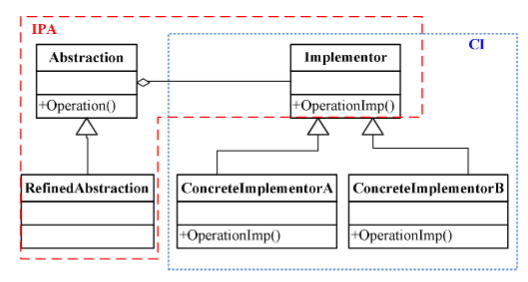
\includegraphics[scale=0.75]{figures/struture_bridge.png}
    \caption{Referenzklassendiagramm des Bridge Patterns mit Submustern}
    \label{fig:structure_bridge}
\end{figure}

Beispielhaft spiegelt die Abbildung \ref{fig:structure_bridge} von Dongjin et al. das definierte Referenzklassendiagramm das Bridge Pattern wieder. Innerhalb dieses Klassendiagramms werden die Submuster \textbf{IPA} und \textbf{CI} festgelegt. Wie von der Abbildung \ref{fig:structure_bridge} zu entnehmen ist, bestehen die Submuster aus einzelnen Entitäten und deren Assoziationen.
Innerhalb der Klassendiagramme des Quellcodes, welches als Eingabe dient, wird nach solchen Submustern durch Einsatz von Graphenisomorphie gesucht~\cite[S. 584]{6649882}. Im weiteren Verlauf werden identifizierte, relevante Submuster zu einer Kandidatenstruktur verschmolzen. Dabei ist anzumerken, dass nur die Submuster, die im betrachtenden Entwurfsmuster vorkommen, in der Verschmelzung involviert sind.
Als finaler Schritt werden durch Analyse des Verhaltensmusters der Kandidatenstrukturen falsch positiv identifizierte Instanzen herausgefiltert~\cite[S. 584]{6649882}. Quellcode aus vier Open-Source-Software-Systemen dient als Eingabe für dieses Verfahren~\cite[S. 585]{6649882}. 
Zu Evaluierung der Resultate der Methodik wird die Metrik der \textit{Precision} verwendet. Dabei wird das Verhältnis zwischen der Anzahl der positiv falschen identifizierten Instanzen zu der Summe der Anzahl der positiv falsch und falsch positiv klassifizierten Instanzen gebildet~\cite[S. 585]{6649882}. Je höher diese ist, desto besser ist das Ergebnis einzustufen.
Nach eigenständiger Evaluierung von Dongjin et al. wird für alle Software-Systeme für alle betrachten strukturellen Entwurfsmuster eine hohe Rate der \textit{Precision} ermittelt~\cite[S. 586]{6649882}.

%TODO: Add this file:///home/memi/Downloads/Yu,%20Dongjin_%20Zhang,%20Yanyan_%20Ge,%20Jianlin_%20Wu,%20Wei%20-%20[IEEE%202013%20IEEE%2037th%20Annual%20Computer%20Software%20and%20Applications%20Conference%20(COMPSAC)%20-%20Kyoto,%20Japan%20(2013.07.22-2013.07.26)]%20201%20(2013,%20IEEE)%20[10.1109_COMPSAC.2013.92]%20-%20libge.pdf

\pagebreak

\subsection{Machine Learning Ansätze}

Mit der ersten öffentlich zugänglichen Version des Open Source Machine Learning Frameworks TensorFlow am 9. November 2015 wurde der Zugang für praktisch angewandtes Machine Learning für Software-Entwickler erleichtert. Durch TensorFlow wird eine Abstraktionsschicht für das Entwerfen, Trainieren und den Betrieb von Machine Learning Modellen eingeführt. Der vereinfachte Einsatz resultiert mit der Anwendung von Machine Learning in Produkten und in der Forschung. Dies ist auch der Fall für die Erkennung von Design Patterns in Quellcode.
Wie aus Abbildung~\ref{fig:approach_dist} zu entnehmen ist, stellen nach der Untersuchung von Yarahmadi et al. Verfahren, die Machine Learning einsetzen, einen signifikanten Teil dar.
Im Kontext dieser Aussage werden in diesem Abschnitt ausgewählte Verfahren erläutert, die Machine Learning als Teil des Erkennungsprozesses anwenden.
Der Fokus in dieser Sektion liegt neben den angewandten Modellen für die Klassifikation auf dem Format der Eingabe, in der die Quellcode-Dateien für die Klassifikation transformiert werden.

Eine Möglichkeit, um Entitäten aus dem Quellcode wie Klassen oder Schnittstellen und deren Assoziation darzustellen, ist die Darstellung als Klassendiagramme aus der UML-Domäne.
In ihrer Methodik nutzen Wang et al. UML-Klassendiagramme als Grundlage und modifizieren diese mit der Inkorporation von Farb- und Symbolcodierungen. Dieses Format benennen Wang et al. \textit{Colored UML}~\cite[S. 6]{app12178718}.

\begin{figure}[h]
    \centering
    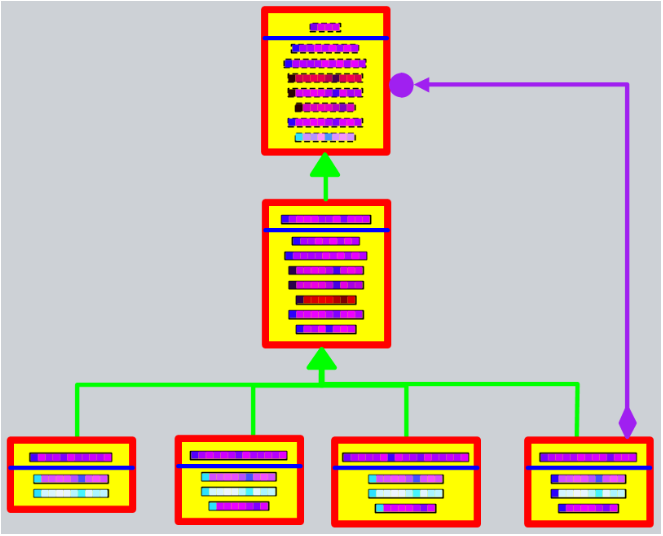
\includegraphics[scale=0.75]{figures/colored_uml.png}
    \caption{\textit{Colored UMl} für eine Mikroarchitektur}
    \label{fig:colored_uml}
\end{figure}

Die Abbildung \ref{fig:colored_uml} zeigt von Wang et al. erstelltes Exemplar für \textit{Colored UML}~\cite[S. 11]{app12178718}. Wie aus der Abbildung \ref{fig:colored_uml} zu entnehmen ist, werden Bezeichner, Modifizierer und Assoziationen farblich und/oder symbolisch encodiert.
Hierbei ist zu erwähnen, dass die Encodierung von Klassenattributen im Kontext dieser Arbeit von Wang et al, nicht berücksichtigt wird.
Die Rechtecke, die in Sektionen aufgeteilt sind, beschreiben die Klassen im Klassendiagramm. Die obere Sektion beinhaltet den Klassenbezeichner und dessen Modifizierer, während die untere Sektion die Methodennamen und deren Modifizierer beinhaltet. 
Jeder Bezeichner wird als Sequenz von Charakteren aufgefasst, in welchem für jeden Charakter algorithmisch eine Farbe aus dem Rot-Grün-Blau-Farbraum ermittelt wird~\cite[S. 9, S. 10]{app12178718}.
Modifizierer für Methoden werden als Teil der Charaktersequenz betrachtet und mitencodiert, während die Modifizierer für Klassen im Rand des Rechtecks encodiert werden, welches den Klassenbezeichner umschließt~\cite[S. 6]{app12178718}.
Die Kanten des Klassendiagramms, welche die Assoziationen zwischen Entitäten darstellen, werden in \textit{Colored UML} farblich annotiert und mit symbolisch an den Enden der Kanten je nach Art der Assoziation encodiert~\cite[S. 6]{app12178718}.

Zunächst werden im ersten Schritt des Prozesses aus Quelldateien durch Software-Werkzeuge UML-Klassendiagramme erstellt, welche im nächsten Schritt in \textit{Colored UML} umgewandelt werden.
Auf den encodierten Quelldaten wird der Bildklassifizierer VGGNet angewendet, welches Features aus der Eingabe als numerischen Vektor mit einer Länge von 1000 extrahiert. Im finalen Schritt dient dieser Feature-Vektor als Eingabe für eine Support Vector Machine, welches die Klassifikation übernimmt, zu welchem Entwurfsmuster die Eingabe zugeordnet werden kann~\cite[S. 13]{app12178718}.
Das hier präsentierte Modell wird für zwölf Design Patterns trainiert~\cite[S. 15]{app12178718}
Für das Training des Modells und die Evaluierung der Resultate des Verfahrens werden drei Open Source Software-Systeme verwendet. Zusätzlich wird das Verfahren mit drei nicht Machine Learning-Verfahren auf \textit{Precision} und \textit{Recall} verglichen~\cite[S. 20]{app12178718}.
Nach eigener Evaluierung von Wang et. al weist das ihrerseits entwickelte Verfahren verglichen zu den anderen Methoden ähnliche oder bessere Klassifizierungsleistung auf~\cite[S. 22]{app12178718}.

\pagebreak

Eine weitere Möglichkeit, um Entwurfsmuster im Quellcode zu ermitteln, ist die Extraktion von Metriken und Maßen aus dem Quellcode, die typisch für eine Instanz des betrachteten Design Pattern sind.
In ihrer Arbeit fokussieren sich Uchiyama et al. auf diesen Punkt und definieren einen Katalog aus Metriken und Maßen, der als Eingabe für einen Klassifizierer verwendet werden.
In dieser Arbeit definieren Uchiyama et al. Design Patterns als eine Summe von Strukturen, die im Kontext des Entwurfsmusters eine Rolle zugeordnet werden~\cite[S. 3]{Uchiyama2014}.
Dabei limitieren sich Uchiyama et al. auf die Erkennung von fünf Entwurfsmustern mit insgesamt 12 Rollen im Quellcode.~\cite[S. 4]{Uchiyama2014}.
Für diese Rollen werden Metriken und Maße ermittelt, die diese charakteristisch beschreiben.
Um die Elemente des Katalogs zu bestimmen, wird in dieser Arbeit die Goal-Question-Metric Methode angewendet~\cite[S. 4]{Uchiyama2014}.
Hierbei werden gezielt Fragen gestellt, mit dem Ziel, die jeweilige Rolle zu bestimmen. Für die Beantwortung dieser Fragen werden Metriken bzw. Maße definiert und als Teil des Katalogs aufgenommen.
Um die zwölf Rollen zu bestimmen, definieren Uchiyama et. al folgende Metriken~\cite[S. 7]{Uchiyama2014}:


\begin{table}[H]
    \centering
    \begin{tabular}{|c|c|}
        \hline
        Abkürzung & Beschreibung\\
        \hline
        NOF & Anzahl der Felder\\
        NSF & Anzahl der statischen Felder\\
        NOM & Anzahl der Methoden\\
        NSM & Anzahl der statischen Methoden\\
        NOI & Anzahl der implementierten Schnittstellen\\
        NOAM & Anzahl abstrakter Methoden\\
        NORM & Anzahl der überschriebenen Methoden\\
        NOPC & Anzahl der privaten Konstruktoren in der Klasse\\
        NOTC & Anzahl der Konstruktoren mit Objektparametern\\
        NOOF & Anzahl der an Feldern mit Objekttypen\\
        NCOF & Anzahl der anderer, die die Klasse/Schnittstelle als Feld referenzieren\\
        NMGI & Anzahl der Methoden, die Instanzen generieren\\
        \hline 
    \end{tabular}
    \caption{Metriken und Maße für Rollen nach Uchiyama et al.}
    \label{table:metrics}
\end{table}

Im ersten Schritt ihrer Methode extrahieren Uchiyama et al. die aus der Tabelle~\ref{table:metrics} definierten Metriken für jede Entität aus den Quelldateien. 
Diese Metriken werden als Vektor aufgefasst und diese werden als Eingabe für einen Klassifizierer verwendet, welche die Rollenzuweisung übernimmt~\cite[S. 5]{Uchiyama2014}.
Bei dem in dieser Methodik angewandten Klassifizierter handelt es sich um ein neuronales Netzwerk~\cite[S. 4]{Uchiyama2014}.
Die Ausgabe des Klassifizierers sind Werte, die angeben, mit welcher Sicherheit der Feature-Vektor zu der jeweiligen Rolle zugeordnet werden kann~\cite[S. 5]{Uchiyama2014}.
Anhand dieser Ausgabe werden die Rollen mit dem höchsten Konfidenzwert als Eingabe für die Bestimmung des Entwurfsmusters genommen. Unter der Berücksichtigung der Relationen der Rollen in dem Entwurfsmuster wird ein Übereinstimmungswert ermittelt, der angibt, mit welcher Wahrscheinlichkeit die Rollen zu dem jeweiligen Design Pattern passen.~\cite[S. 6]{Uchiyama2014}. Je höher dieser Wert, desto höher die Konfidenz, dass es sich hierbei um das Entwurfsmuster handelt.
Für das Training ihres Klassifizierers nutzen Uchiyama et al. 60 Instanzen aus klein-skalierten Software-Systemen und 158 aus drei größeren Open Source Software-Systemen.~\cite[S. 7]{Uchiyama2014}
Für die Evaluierung der Methode bedienen sich Uchiyama et. al den Metriken der \textit{Precision} und \textit{Recall} und ermitteln diese für ihr Verfahren.
Dabei werden für Instanzen aus klein-skalierten Software-Systemen bessere \textit{Precison}- und \textit{Recall}-Werte erzielt, verglichen zu den Werten für Instanzen aus den Open Source Software-Systemen~\cite[S. 8]{Uchiyama2014}

\smallbreak

Durch Charakterisierung der Klassen, Schnittstellen und Objekte durch Metriken und Maße sind zwar Rückschlüsse auf Struktur und Verhalten möglich, jedoch wird der lexigrafische und syntaktische Aspekt nicht mit berücksichtigt.
Um dagegenzuwirken, präsentieren Nazar et. al in ihrer Arbeit ihre Methode namens DPD\textsubscript{F}, die diese Aspekte des Quellcodes mitberücksichtigt~\cite[S. 1]{Nazar2020}.
Initial wird aus dem Quellcode durch statische Codeanalyse folgende Metriken extrahiert~\cite[S. 5]{Nazar2020}:

\begin{table}[H]
    \begin{tabular}{|c|c|}
        \hline
        Featurebezeichner & Beschreibung\\
        \hline
        ClassName & Name der Java Klasse\\
        ClassModifiers & Public, Protected und Private-Schlüsselwörter\\
        ClassImplements & Binäres Features (0/1), falls eine Schnittstelle implementiert wird\\ 
        ClassExtends & Binäres Features (0/1), ob Klasse von einer anderen vererbt\\
        MethodName & Methodenname in der Klasse\\
        MethodReturnType & Typ des Rückgabewerts einer Methode\\
        MethodBodyLineType & Art des Ausdrucks (z.B Variablenzuweisung, Boolean-Ausdruck)\\
        MethodNumVariables & Anzahl der Variablen/Attribute in der Klasse\\
        MethodNumMethods & Anzahl der Methodenaufrufe in der Klasse\\
        MethodsNumLine & Anzahl der Zeilen in Methode\\
        MethodIncomingMethod & Anzahl an Methoden, die in eine Methode aufruft\\
        MethodIncomingName & Name der Methoden, die von der Methode aufgerufen werden\\
        MethodOutgoingMethod & Anzahl ausgehender Methoden\\
        MethodOutgoingName & Name der ausgehenden Methoden\\
        \hline  
    \end{tabular}
    \caption{Extrahierte Features für DPD\textsubscript{F}}
    \label{table:dpdf_features}
\end{table}

Die ersten vier in der Tabelle \ref{table:dpdf_features} aufgelisteten Features werden pro Klasse ermittelt, während die restlichen elf für jede Methode in der Klasse bestimmt werden.
Jedes dieser Features wird als eine Auflistung von Schlüssel-Werte-Paaren in natürlicher Sprache formuliert.
Da die Ermittelung der Metriken für jede Methodendefinition durchgeführt wird, werden Features der Klasse in der Methodenevaluierung wiederholt.
Jede Evaluierung wird als Eintrag in einer Textdatei zusammengefasst. Das dabei entstehende Format wird von Nazar at al. als Syntactic and Lexical Representation (SSLR) benannt~\cite[S. 1]{Nazar2020}.
Um dieses Format in eine numerische Form zu bringen, wird SSLR als Eingabe für das Embedding-Modell Word2Vec verwendet, welches für jedes Token in der Eingabe durch Einbezug der umgebenden Tokens einen numerischen Vektor mit einer Länge von 100 determiniert, welches das jeweilige Token repräsentiert~\cite[S. 6]{Nazar2020}.
Die resultierenden Vektoren dienen als Eingabe für einen Random Forest Classifier, welches das meist passende Entwurfsmuster bestimmt~\cite[S. 7]{Nazar2020}.
Für das Training der Modelle und Evaluierung von DPD\textsubscript{F} wird ein eigener Korpus angelegt, bestehend aus Quelldateien aus \textit{Github Java Corpus}. Für die Evaluation und das Training werden zwölf Entwurfsmuster mit je 100 Instanzen aus dem Korpus genutzt, die durch Crowdsourcing identifiziert wurden~\cite[S. 4]{Nazar2020}.
Die Beurteilung der Resultate erfolgt durch die Bestimmung der \textit{f1}-, \textit{Precision}- und \textit{Recall}-Werte wird für jedes betrachtete Design Pattern. Nach eigener Evaluation erreicht ihre Methode mit dem selbsterstellten Datensatz im Durchschnitt einen \textit{Precision}-Wert von über 80\% und einen \textit{Recall}-Wert von 79\%~\cite[S. 8]{Nazar2020}.


\subsection{Query Ansätze}

Eine weitere Möglichkeit, um Design Patterns in Quellcode zu identifizieren, ist durch das Stellen von Anfragen an das Software-System.
Die Antwort auf die gestellte Anfrage ist dabei solch eine, die die in der Anfrage formulierten Bedingungen am besten befriedigt.
Solch einen Ansatz verfolgen Mäder et al. in ihrer Methodik. Dabei liegt der Fokus in ihrer Methode auf Annotationen im Quellcode,
die Aufschlüsse auf mögliche Entwurfsmuster geben. In ihrer Arbeit definieren Mäder et al. Annotation als Teil des Quellcodes, die keine direkte Einwirkung auf Programmsemantik haben~\cite[S. 521]{Ghula-2010} und bieten gleichzeitig zusätzliche Informationen für statische Analyse durch Software-Werkzeuge und für das Verständnis des Software-Systems an.
Initial wird ein Katalog von Annotationen definiert, welche manuell von Software-Entwicklern in Quellcode des Software-Systems aufgenommen wird~\cite[S. 521]{Ghula-2010}.

\begin{figure}[h]
    \centering
    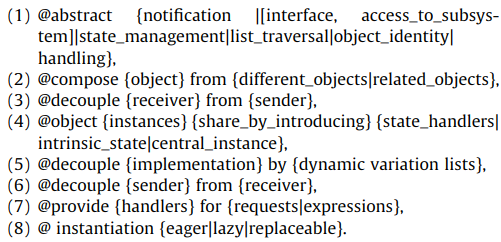
\includegraphics{figures/annotations.png}
    \caption{Ausschnitt an Annoation von Guhlam et al.}
    \label{fig:annotations}
\end{figure}

Abbildung \ref{fig:annotations} zeigt einen Ausschnitt des Annotationskatalogs, welcher im Kontext der Arbeit definiert wird. Dabei sind diese Annotationen so bestimmt, dass diese Informationen über die Struktur und Verhalten des Software-Artefakts widerspiegeln.
Der annotierte Quellcode wird im weiteren Verlauf durch das Software-Werkzeug Enterprise Architekt prozessiert. Dieses Werkzeug generiert ein Modell des Quellcodes und inkludiert die Beziehungen zwischen Software-Artefakten~\cite[S. 521]{Ghula-2010}. Informationen über Aggregation, Delegation und Freundschaften sind nicht Teil dieses Modells~\cite[S. 521]{Ghula-2010}.
Um die Existenz von Entwurfsmustern zu erkennen, wird ein Katalog an Regeln definiert, die verschiedene Aspekte von Design Patterns durch Mitberücksichtigung der Annotationen widerspiegelt~\cite[S. 523]{Ghula-2010}. Diese Regeln werden in SQL-Anfragen und reguläre Ausdrücke transformiert und in Sets von Regeln aufgeteilt, die auf die Existenz des zugewiesenen Design Patterns überprüfen~\cite[S. 523]{Ghula-2010}.  
Zu der Evaluierung ihrer Methode vergleichen Mäder et al. ihre Methode mit zwei anderen Verfahren. Dabei wird verglichen, welche Entwurfsmuster diese erkennen~\cite[S. 525]{Ghula-2010}.
Konkrete Metriken sind zu dem Zeitpunkt des Verfassens ihrer Arbeit nicht verfügbar~\cite[S. 525]{Ghula-2010}.

\pagebreak

Anstatt die Modellierung an ein professionelles Software-Werkzeug zu delegieren, entwerfen Stencel et al. ein eigenes Metamodell, wonach Entitäten aus dem Quellcode und ihre Relationen zueinander modelliert werden~\cite[S. 27]{stencel-2008}.
Dabei besteht das Metamodell aus Kernelementen wie types, attributes operations und instances und strukturellen und verhaltensbezogenen Relationen zwischen diesen Kernelementen. Sowohl die Kernelemente als auch die Relationen in diesem Metamodell sind möglichst ähnlich nach dem aus der objektorientierter Programmierung bekannten Verständnis definiert~\cite[S. 27]{stencel-2008}.
Jedes Design Pattern, das in dieser Arbeit betrachtet wird, wird von Stencel et al. in ihrem  Metamodell encodiert~\cite[S.28 - 29]{stencel-2008}. Diese dienen als Referenz für die Erkennung des jeweiligen Entwurfsmusters im Quellcode und werden als Grundlage für SQL-Anfragen genutzt~\cite[S. 29]{stencel-2008}.
In der Implementierung der Methode wird durch Strukturanalyse, Analyse des Datenflusses und Analyse der Methodenaufrufe Artefakte in das Metamodell transformiert und in einer relationalen Datenbank abgelegt.
Durch die SQL-Abfragen wird in der Datenbank nach Instanzen abgefragt, die die von der Referenzdefinition bereitgestellten Bedingungen erfüllen.
Zu Evaluierung vergleichen Stencel et al. ihre Methode mit zwei anderen und überprüfen anhand von Software-Systemen, welche Entwurfsmuster erkannt werden~\cite[S. 30]{stencel-2008}.
Als Resultat erkennt das hier erläuterte Verfahren mehr Instanzen an als die anderen Methoden~\cite[S. 29]{stencel-2008}.

\subsection{Diverse Ansätze}

%%TODO: Explain 2-4 other misc approaches; I AM SO FUCKING DONE
In ihrer Arbeit präsentieren Kramer et al. eine der frühesten Verfahren, um Entwurfsmuster in Quellcode zu erkennen.
Mit der Absicht, die Wartbarkeit von Software-Systemen zu verbessern, nutzen die Kramer et al. die Programmiersprache PROLOG, um 
Design Patterns als einzelne Regeln zu repräsentieren~\cite[S. 2]{Krammer-1996}. Diese dienen als Referenz im weiteren Verlauf der Methode.
Initial wird der zu verarbeitende Quellcode durch ein Software-Werkzeug in ein Object-Modelling Technique Diagramm transformiert und im nächsten Schritt wird das erstellte Diagramm in PROLOG-Code übersetzt.
Die als Referenz genutzten Definitionen der Entwurfsmuster dienen als Anfrage, die in dem transformierten Quellcode nach Instanzen des jeweiligen Design Patterns suchen~\cite[S. 2]{Krammer-1996}.
Zu Evaluierung werden von Kramer et al. die Definitionen für die Design Patterns Adapter, Bridge, Decorater und Proxy angelegt und die Methode an vier C++-Bibliotheken angewendet.
Nach eigener Evaluierung von Kramer et al. erzielt die Methode einen \textit{Precision}-Wert zwischen 14\% und 50\%~\cite[S. 7]{Krammer-1996}.

Anstatt ein Verfahren von Grund aus neu zu entwerfen, bedienen sich Binun et al. in ihrer Methode auf bereits etablierte Software-Werkzeuge und Methoden.
Sie erläutern, dass unterschiedliche Verfahren die einzelnen betrachteten Entwurfsmuster unterschiedlich präzise erkennen~\cite[S.15 - 17]{binun2009}.
In ihrer Methode wird die Ausgabe von fünf Verfahren zu einem finalen Wert zusammengefasst, der angibt, mit welcher Wahrscheinlichkeit es sich um das determinierte Design Pattern handelt.
Falls die einzelnen Methoden oder Werkzeuge die Eingabe unterschiedlich klassifizieren, wird versucht, durch die Identifikation einzelner Rollen im Quellcode das Entwurfsmuster zu rekonstruieren und dadurch die Eingabe einem Entwurfsmuster zuzuordnen~\cite[S. 15 - 16]{binun2009}.
Für die Evaluierung bedienen sie sich zwölf Software-Systeme als Eingabe für ihre Methode. In diesen wird nach Instanzen von fünf Entwurfsmustern gesucht~\cite[S. 9, S. 23]{binun2009}.
Nach eigener Evaluierung von Binun et al. werden drei von fünf Entwurfsmustern mit einem \textit{Precision}-Wert von über 70\% erkannt, während für die restlichen zwei mehrheitlich von den aggregierten Methoden nicht erkannt werden~\cite[S. 22]{binun2009}.

